\section{Results}

\subsection{Main empirical takeaway}

The strongest overall conclusion is not that one model family wins everywhere.
Instead, the benchmark supports \emph{age-aware model selection under
structural and observation uncertainty}. Strong hand-designed baselines remain
competitive or superior for several series, while constrained discovery is
clearly useful for selected age groups. Observation structure also matters:
once the discovery grammar is allowed to search over delayed observation, it
selects \texttt{delayed\_I} in multiple age groups, but it still does not
select \texttt{H} or \texttt{I+H} in the current single-season benchmark.

\subsection{Observation-aware multi-seed point-forecast results}

Table~\ref{tab:obs-aware-summary} summarizes the current observation-aware
five-seed aggregate. The table is based on
\texttt{artifacts\_multiseed\_age\_robustness\_observation/} and reflects the
latest non-LLM control benchmark.

\begin{table}[H]
\centering
\caption{Observation-aware five-seed recommendation summary. The
recommendation column reports the modal recommendation over seeds, while the
``best test'' and ``best rolling'' columns summarize which model family most
often wins the held-out test split and rolling-origin evaluation.}
\label{tab:obs-aware-summary}
\begin{tabularx}{\textwidth}{>{\raggedright\arraybackslash}p{1.45cm} >{\raggedright\arraybackslash}p{3.0cm} >{\raggedright\arraybackslash}p{2.7cm} >{\raggedright\arraybackslash}p{2.7cm} X}
\toprule
Series & Recommended model & Best test pattern & Best rolling pattern & Interpretation \\
\midrule
Overall & \texttt{deterministic\_seir} & \texttt{delayed\_observation\_seir} wins $4/5$ seeds & split between deterministic and delayed baselines & Observation-aware manual baselines dominate discovery on the overall aggregate. \\
0--4 yr & \texttt{constrained\_structure\_discovery} & discovery wins $5/5$ seeds & discovery wins $5/5$ seeds & Clearest stable discovery success case in the repository. \\
5--17 yr & \texttt{constrained\_structure\_discovery} & discovery wins $4/5$ seeds & \texttt{probabilistic\_seir} wins $5/5$ seeds & Strong held-out discovery result, but rolling-origin stability still favors the probabilistic baseline. \\
18--49 yr & \texttt{deterministic\_seir} & split across deterministic, delayed, and hospitalized baselines & deterministic wins $3/5$ seeds & Discovery is not competitive; the relevant comparison is among strong manual baselines. \\
50--64 yr & \texttt{delayed\_observation\_seir} & \texttt{hospitalized\_seihr} wins $3/5$ seeds & delayed baseline wins $4/5$ seeds & Fair hospitalization-aware baselines largely replace discovery as the main story. \\
$\geq$65 yr & \texttt{deterministic\_seir} & deterministic wins $3/5$ seeds & discovery wins $4/5$ seeds & The older-adult series remains split-sensitive between held-out and rolling-origin criteria. \\
\bottomrule
\end{tabularx}
\end{table}

The numerical aggregate reinforces this qualitative view. For the overall
series, \texttt{delayed\_observation\_seir} achieves mean test
MAE~\num{0.035056}, outperforming \texttt{deterministic\_seir}
(\num{0.035205}) and discovery (\num{0.036967}). For \texttt{0-4 yr},
discovery remains decisively best with mean test MAE~\num{0.090596} and mean
rolling MAE~\num{0.123344}. In contrast, for \texttt{50-64 yr},
\texttt{hospitalized\_seihr} wins held-out test most often while
\texttt{delayed\_observation\_seir} dominates rolling-origin MAE, making this
age group far less of a clean discovery-wins case than it appeared before the
fair-baseline expansion.

\begin{figure}[H]
\centering
\begin{subfigure}[t]{0.49\textwidth}
  \centering
  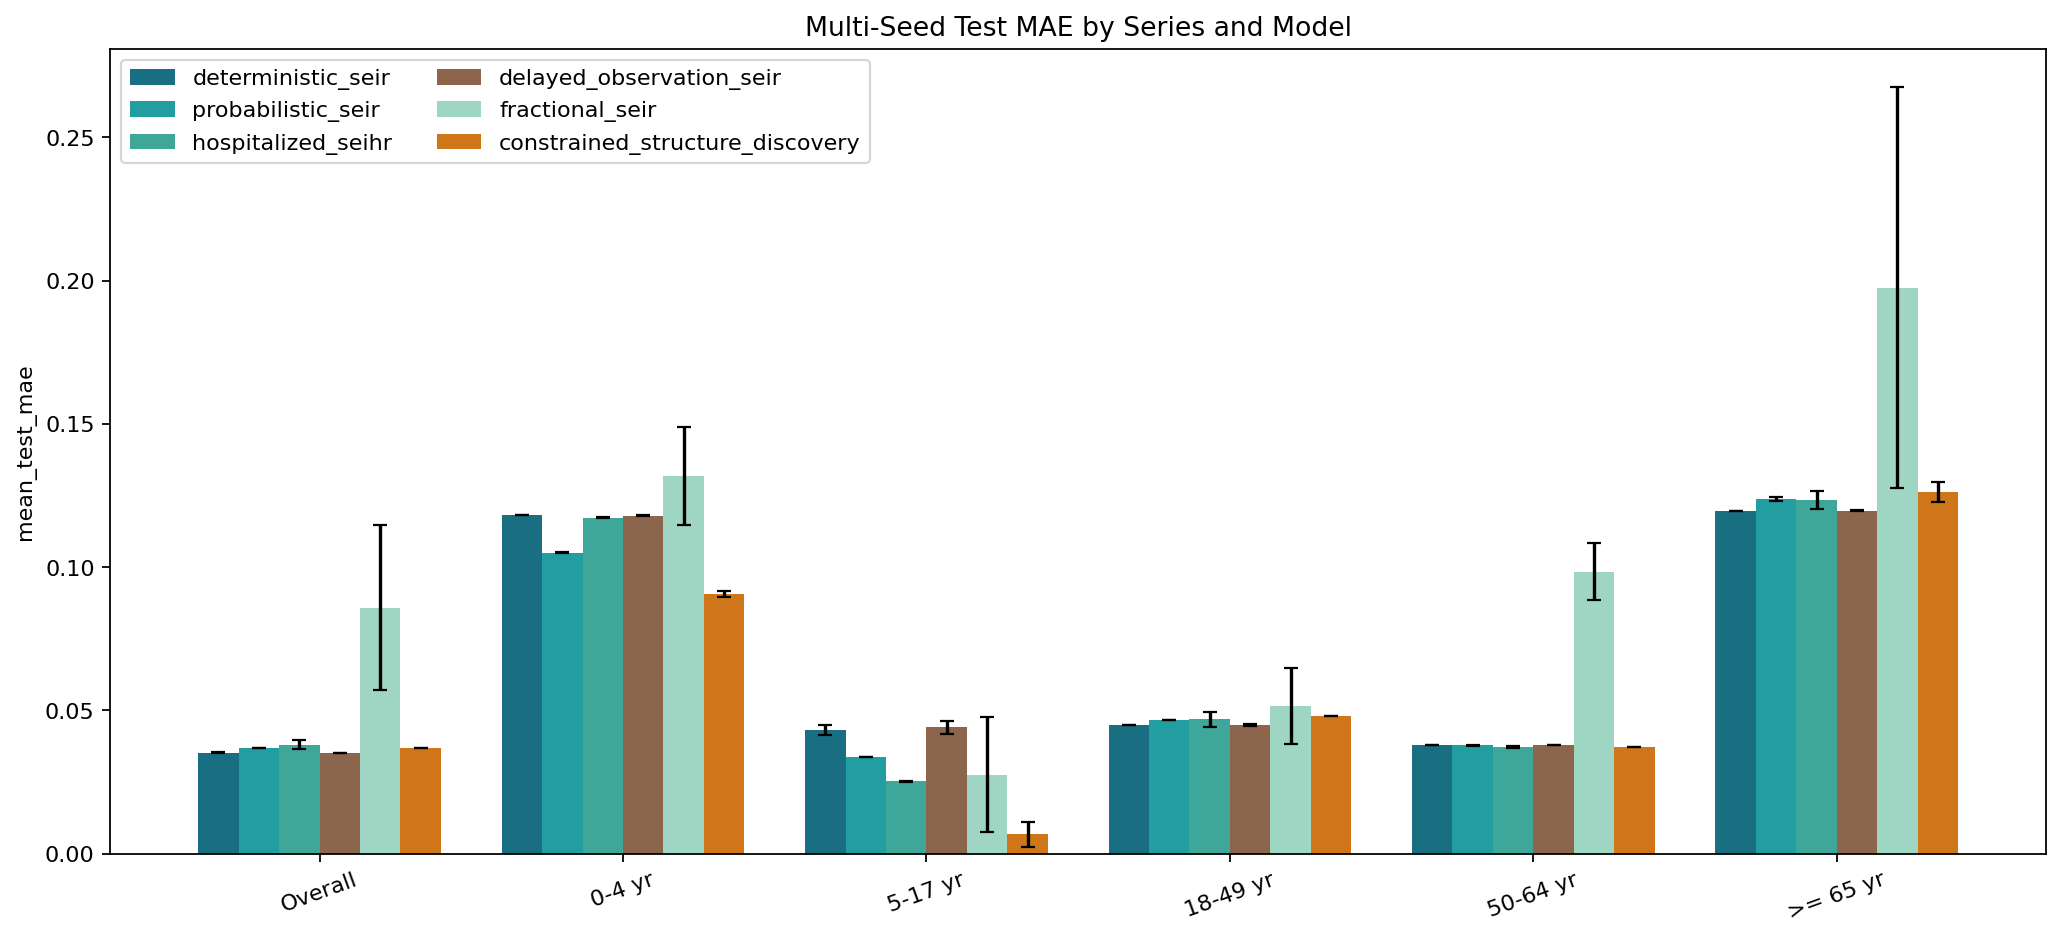
\includegraphics[width=\linewidth]{../artifacts_multiseed_age_robustness_observation/multiseed_test_mae_errorbars.png}
  \caption{Held-out test MAE across five seeds.}
\end{subfigure}
\hfill
\begin{subfigure}[t]{0.49\textwidth}
  \centering
  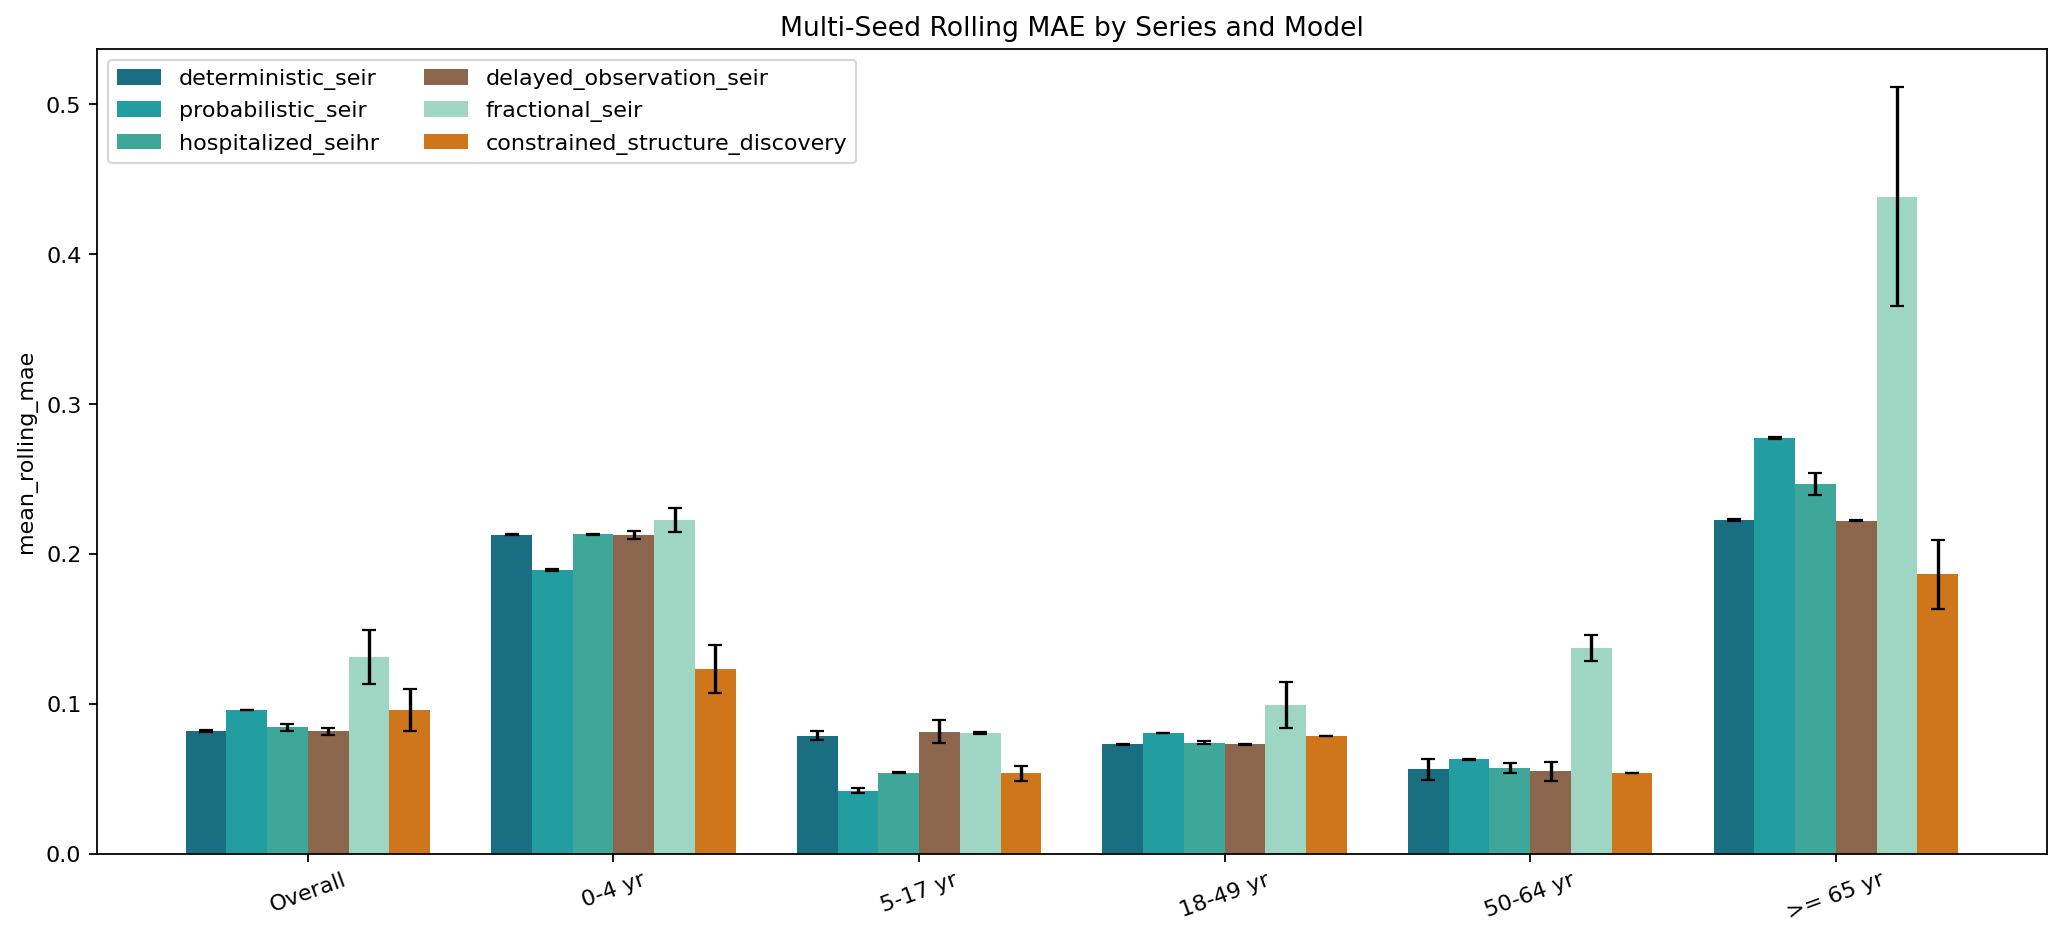
\includegraphics[width=\linewidth]{../artifacts_multiseed_age_robustness_observation/multiseed_rolling_mae_errorbars.png}
  \caption{Rolling-origin MAE across five seeds.}
\end{subfigure}
\caption{Observation-aware five-seed robustness plots. Error bars summarize
between-seed variability.}
\label{fig:obs-aware-multiseed}
\end{figure}

\subsection{Objective-aware policy interpretation}

The five-seed aggregate also benefits from a tie-aware policy layer. Rather
than forcing a single recommendation whenever one mean error is numerically
smallest, we define a practical tie separately for held-out test MAE and
rolling-origin MAE:
\[
|m - m^\star| \leq \max(0.001, 0.02 m^\star),
\]
where $m^\star$ is the best mean metric for the current series and objective.
Within each tie set, models are ranked by win rate, between-seed variability,
parameter count, and simplicity priority. This produces
\texttt{test\_policy\_model}, \texttt{rolling\_policy\_model}, and, when
possible, a shared \texttt{parsimony\_policy\_model}.

This policy layer changes how the benchmark should be interpreted. It shows
that $4/6$ series have different held-out-test and rolling-origin policy
winners, but only two series remain fully objective-dependent with no shared
parsimonious compromise. The clean cases are still informative:
\texttt{0--4 yr} remains a discovery win under both objectives, while
\texttt{18--49 yr} collapses to a deterministic recommendation once practical
ties are acknowledged. More interestingly, \texttt{Overall} becomes a
practical tie between \texttt{deterministic\_seir} and
\texttt{delayed\_observation\_seir}, with the deterministic model preferred as
the simpler shared compromise. Likewise, \texttt{50--64 yr} has different test
and rolling winners, yet discovery remains inside both tie sets and therefore
survives as the parsimonious compromise even after fair hospitalization-aware
baselines are added.

The implication is that the current non-LLM benchmark should be described not
only as age-aware but also as objective-aware. Some series genuinely reward one
model over another, but several series are better interpreted as practical ties
whose final recommendation depends on whether the user prioritizes held-out
split accuracy, rolling-origin stability, or model simplicity.

\subsection{Discovery structure and observation semantics}

Table~\ref{tab:discovery-structures} summarizes the structures selected by the
observation-aware discovery grammar over five seeds.

\begin{table}[H]
\centering
\caption{Selected discovery structures in the observation-aware five-seed
benchmark. Frequencies are computed over the five random seeds.}
\label{tab:discovery-structures}
\begin{tabularx}{\textwidth}{>{\raggedright\arraybackslash}p{1.45cm} >{\raggedright\arraybackslash}p{4.4cm} >{\raggedright\arraybackslash}p{1.6cm} X}
\toprule
Series & Dominant selected structure(s) & Frequency & Interpretation \\
\midrule
Overall & \texttt{SIR|fractional=0|obs=I} & $1.0$ & Discovery stays simple when richer observation maps are unnecessary. \\
0--4 yr & \texttt{SEIRS|obs=I} plus delayed variants with delay $1$ and $2$ & $0.6$ for \texttt{obs=I}; $0.4$ delayed combined & Discovery remains structure-rich and occasionally uses delayed observation in children. \\
5--17 yr & \texttt{SEIRS} family with \texttt{obs=I}, \texttt{delayed\_I|delay=2}, and \texttt{delayed\_I|delay=3} & mixed & Discovery explores delay here, but the selected family remains SEIRS in every seed. \\
18--49 yr & \texttt{SIR|fractional=0|obs=I} & $1.0$ & Observation search does not force extra complexity for this adult group. \\
50--64 yr & \texttt{SIR|fractional=0|obs=I} & $1.0$ & Even after observation-grammar expansion, discovery selects the same simple latent structure. \\
$\geq$65 yr & \texttt{SEIRS|fractional=1|obs=delayed\_I|delay=2} and \texttt{SEIRS|fractional=1|obs=I} & $0.6$ delayed, $0.4$ \texttt{I} & Older adults are the strongest case where delayed observation emerges stably from discovery. \\
\bottomrule
\end{tabularx}
\end{table}

Two points are especially important.

\paragraph{Delayed observation emerges without LLMs.}
The expanded grammar now allows the non-LLM discovery loop to recover explicit
observation delay. In the current benchmark, \texttt{delayed\_I} is selected in
children and older adults, including $3/5$ seeds for the
$\geq$65-yr series.

\paragraph{Hospitalization observation is not selected.}
No selected discovery winner uses \texttt{obs=H} or \texttt{obs=I+H}. This
does not imply that hospitalization-aware observation is universally useless:
the manual \texttt{hospitalized\_seihr} baseline remains competitive in several
age groups. Rather, it means that in the current proof-of-concept season, the
non-LLM search finds stronger evidence for delayed infectious observation than
for directly observing the hospitalized compartment.

\subsection{Age-prior ablation}

The observation-aware no-age-prior multi-seed rerun produced the same:
\begin{itemize}[leftmargin=1.5em]
\item \texttt{multiseed\_model\_summary.csv},
\item \texttt{multiseed\_age\_group\_recommendation.csv}, and
\item \texttt{multiseed\_discovery\_structure\_frequency.csv}
\end{itemize}
as the corresponding age-prior-enabled run.

More concretely, the derived comparison tables show:
\begin{itemize}[leftmargin=1.5em]
\item no change in recommended model mode for any of the six series,
\item no change in dominant discovery structure for any series,
\item no change in dominant observation-map mode for any series,
\item no change in dominant delay mode for any series, and
\item zero difference in aggregate discovery test MAE and aggregate discovery
rolling MAE for all six series.
\end{itemize}

This result matters because it rules out a simple confound: the delayed
observation structures are not appearing merely because the search was given an
age-specific structural preference. Instead, the current evidence suggests that
the observation-aware discovery results are driven by the data and the
validation-based search objective rather than by the age prior.

\subsection{Uncertainty calibration}

Although the main emphasis of the current paper core is on point forecasting,
the uncertainty pipeline is already mature enough to report a stable default.
Benchmark-level conformal calibration compares five calibration kinds and three
validation-only winner rules. The current selected rule is the balanced
\texttt{v3} rule.

\begin{table}[H]
\centering
\caption{Comparison of validation-only conformal winner rules. Lower is better
for all three metrics.}
\label{tab:conformal-rules}
\begin{tabular}{lccc}
\toprule
Rule & Mean absolute coverage gap & Mean interval score & Mean width \\
\midrule
v1 & \num{0.189394} & \num{0.460618} & \num{0.451670} \\
v2 & \num{0.183838} & \num{0.484247} & \num{0.473100} \\
v3 & \num{0.184343} & \num{0.465319} & \num{0.456298} \\
\bottomrule
\end{tabular}
\end{table}

The practical interpretation is that v1 is too interval-score-driven, v2 is
too coverage-gap-driven, and v3 provides the best current compromise. This is
why the repository now treats benchmark-level conformal v3 as the default
uncertainty postprocessor while keeping point-forecast selection separate.

\subsection{Implications for the next phase}

These experiments tighten the non-LLM story substantially. We now have:
\begin{enumerate}[leftmargin=1.5em]
\item fair hospitalization-aware manual baselines,
\item observation-aware discovery grammar,
\item five-seed robustness analysis,
\item no-age-prior ablation showing the same aggregate result, and
\item a fixed benchmark-level conformal postprocessor.
\end{enumerate}

This means the next phase should not continue to micro-tune non-LLM search.
Instead, the most valuable next step is an \textbf{LLM-V0} experiment in which
the LLM only proposes and critiques candidate structures while the existing
Python pipeline continues to enforce validity, perform fitting, and evaluate
validation-time performance. The current observation-aware non-LLM benchmark is
now strong enough to serve as a credible control condition for that study.
